\documentclass[mathserif,serif]{beamer}
\usepackage{graphicx}
\usepackage{multimedia}
\usepackage{hyperref}
\usetheme{CambridgeUS}
\hypersetup{
    colorlinks=true,
    linkcolor=blue,
    filecolor=magenta,
    urlcolor=cyan,
}

\title[Docker]{Introduction to Docker}
%\subtitle{Why \& How}
\author[Shubham Chaudhary]{Shubham Chaudhary\inst{1}}
\institute[Zomato Media Pvt.~ Ltd.]{\inst{1} Zomato Media Pvt.~ Ltd.~}
\date[February 2018]{Tech Thursdays, February 01, 2018}
\subject{Computer Science}

\begin{document}
    \frame{\titlepage}
    \begin{frame}
        \frametitle{Table of Contents}
        \tableofcontents[currentsection,currentsubsection]
    \end{frame}

    \section{Why}\label{sec:why}
    \subsection{Problem to be solved}\label{subsec:problemToBeSolved}
%    \begin{frame}
%        \frametitle{The Problem and its solution}
%        \begin{itemize}[<+->]
%            \only<1-1> {
%                \begin{block}{Matrix of Hell}\end{block}
%                \makebox[\textwidth]{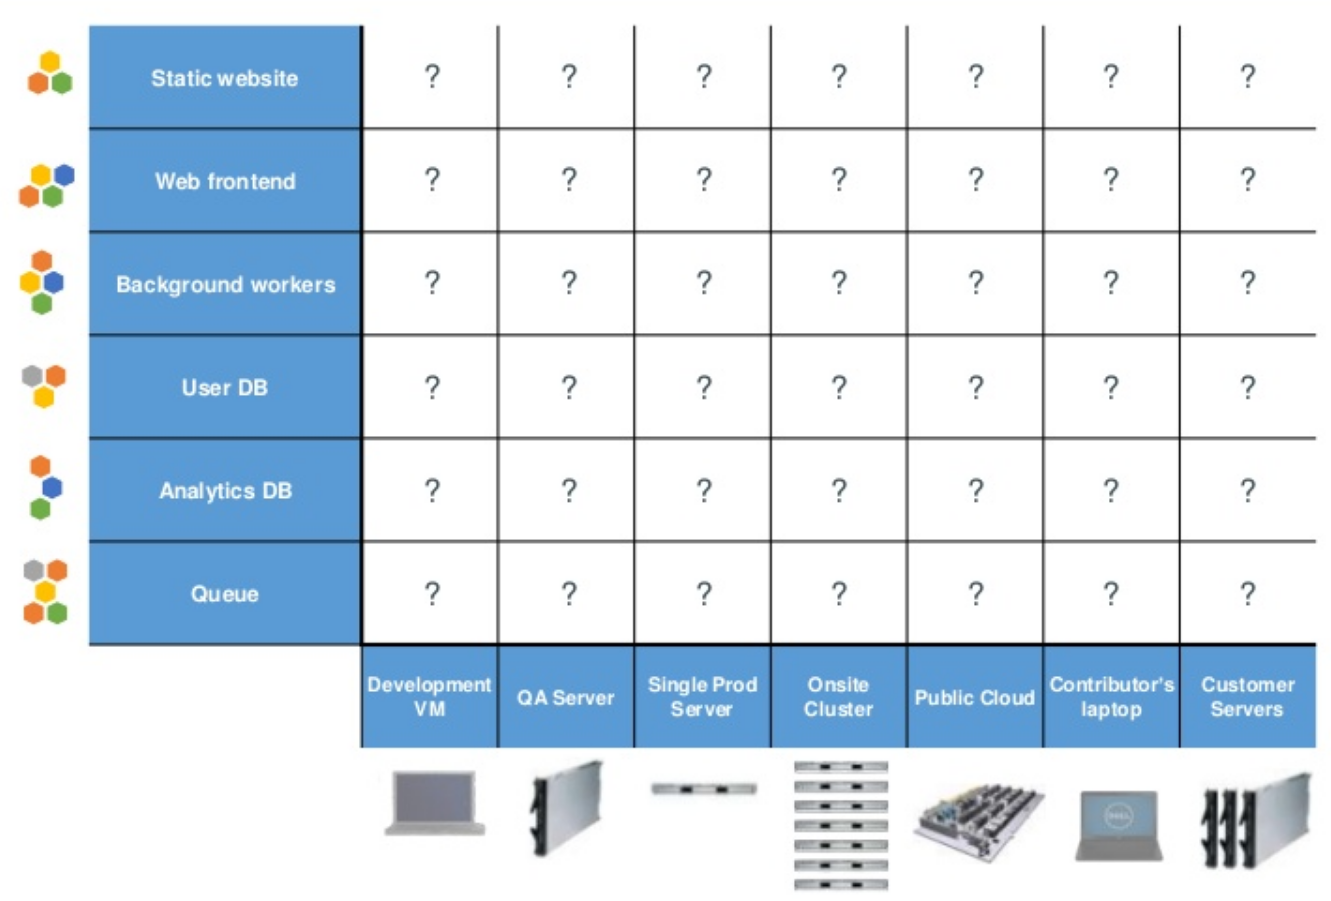
\includegraphics[width=0.80\paperwidth]{docker-zomato/images/matrix_prob.png}}
%            }
%            \only<2-1> {
%            \begin{block}{Docker wasn't the first}\end{block}
%                \makebox[\textwidth]{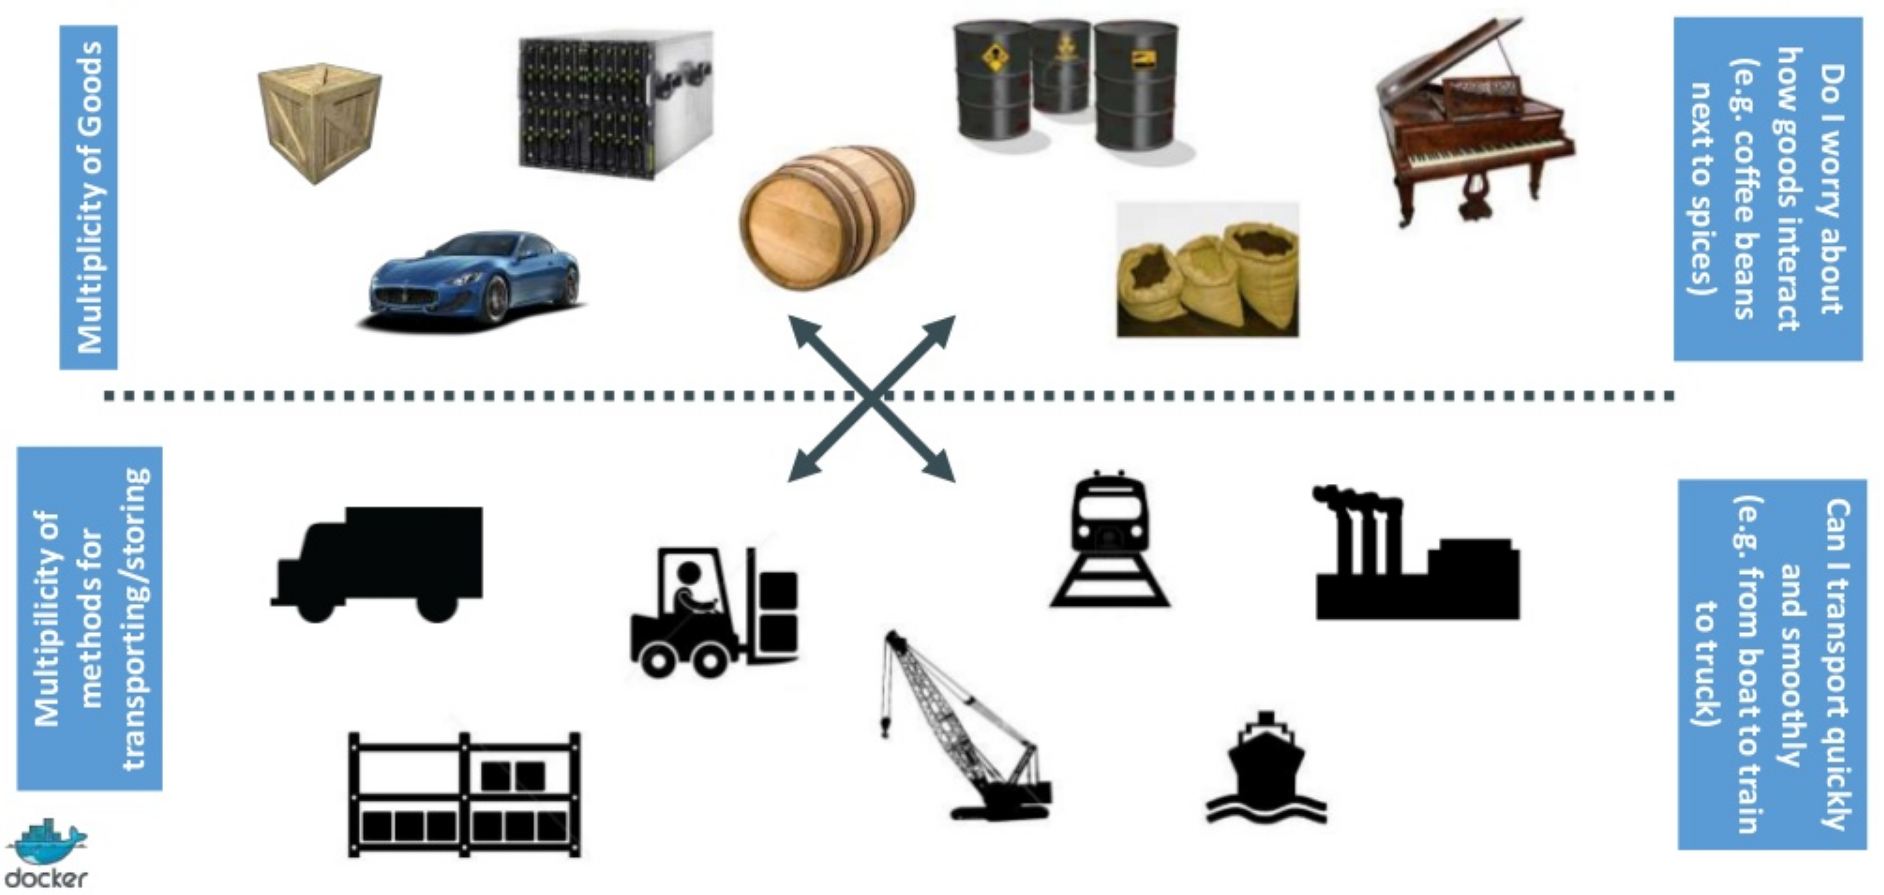
\includegraphics[width=0.80\paperwidth]{docker-zomato/images/cargo_prob.png}}
%            }
%            \only<3-1> {
%            \begin{block}{Similar matrix of hell}\end{block}
%                \makebox[\textwidth]{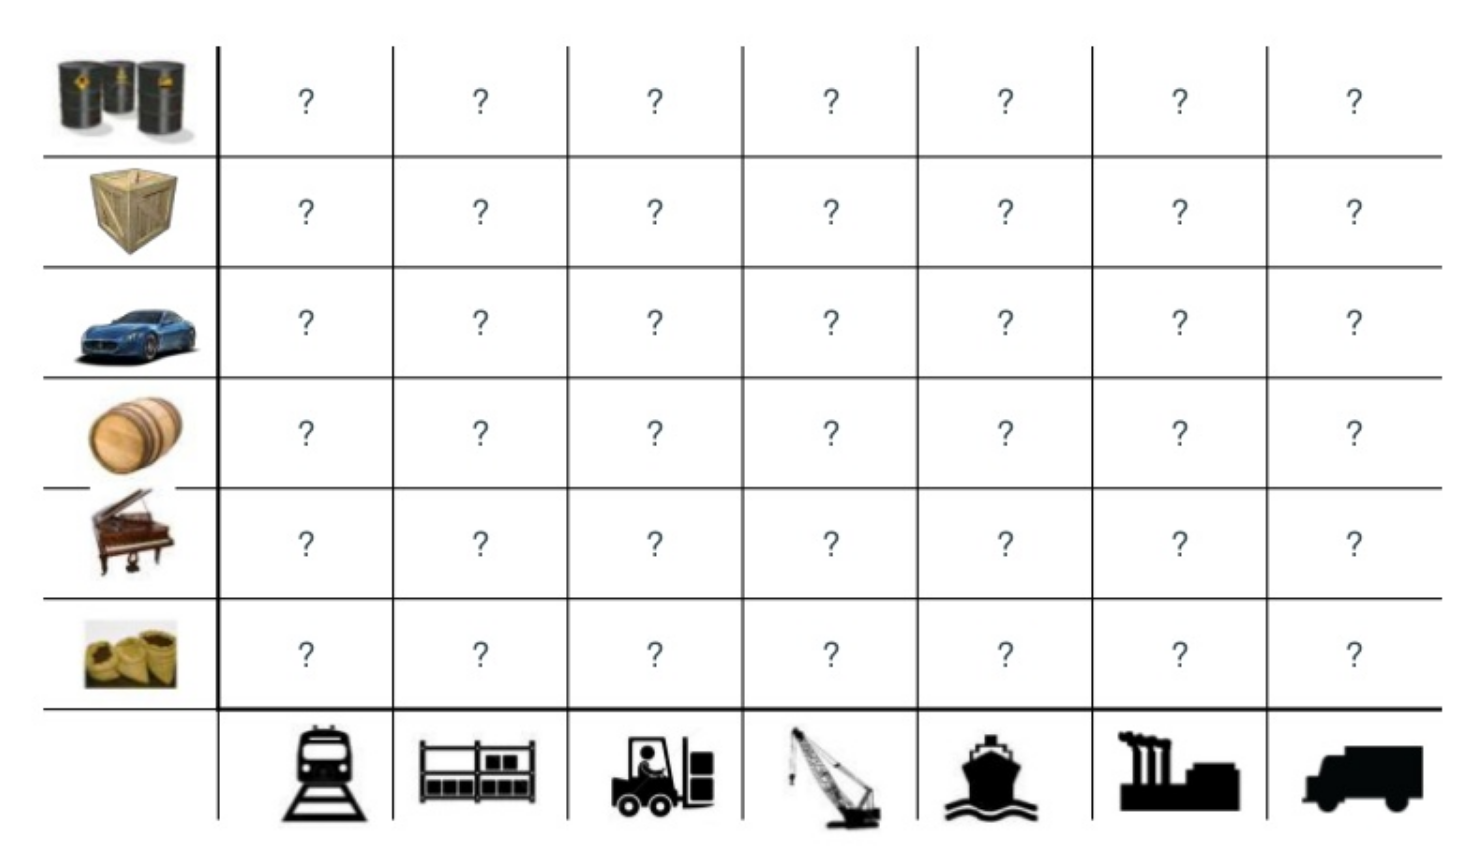
\includegraphics[width=0.80\paperwidth]{docker-zomato/images/cargo_matrix.png}}
%            }
%            \only<4-1> {
%            \begin{block}{Cargo Industry's Solution - Containers}\end{block}
%                \makebox[\textwidth]{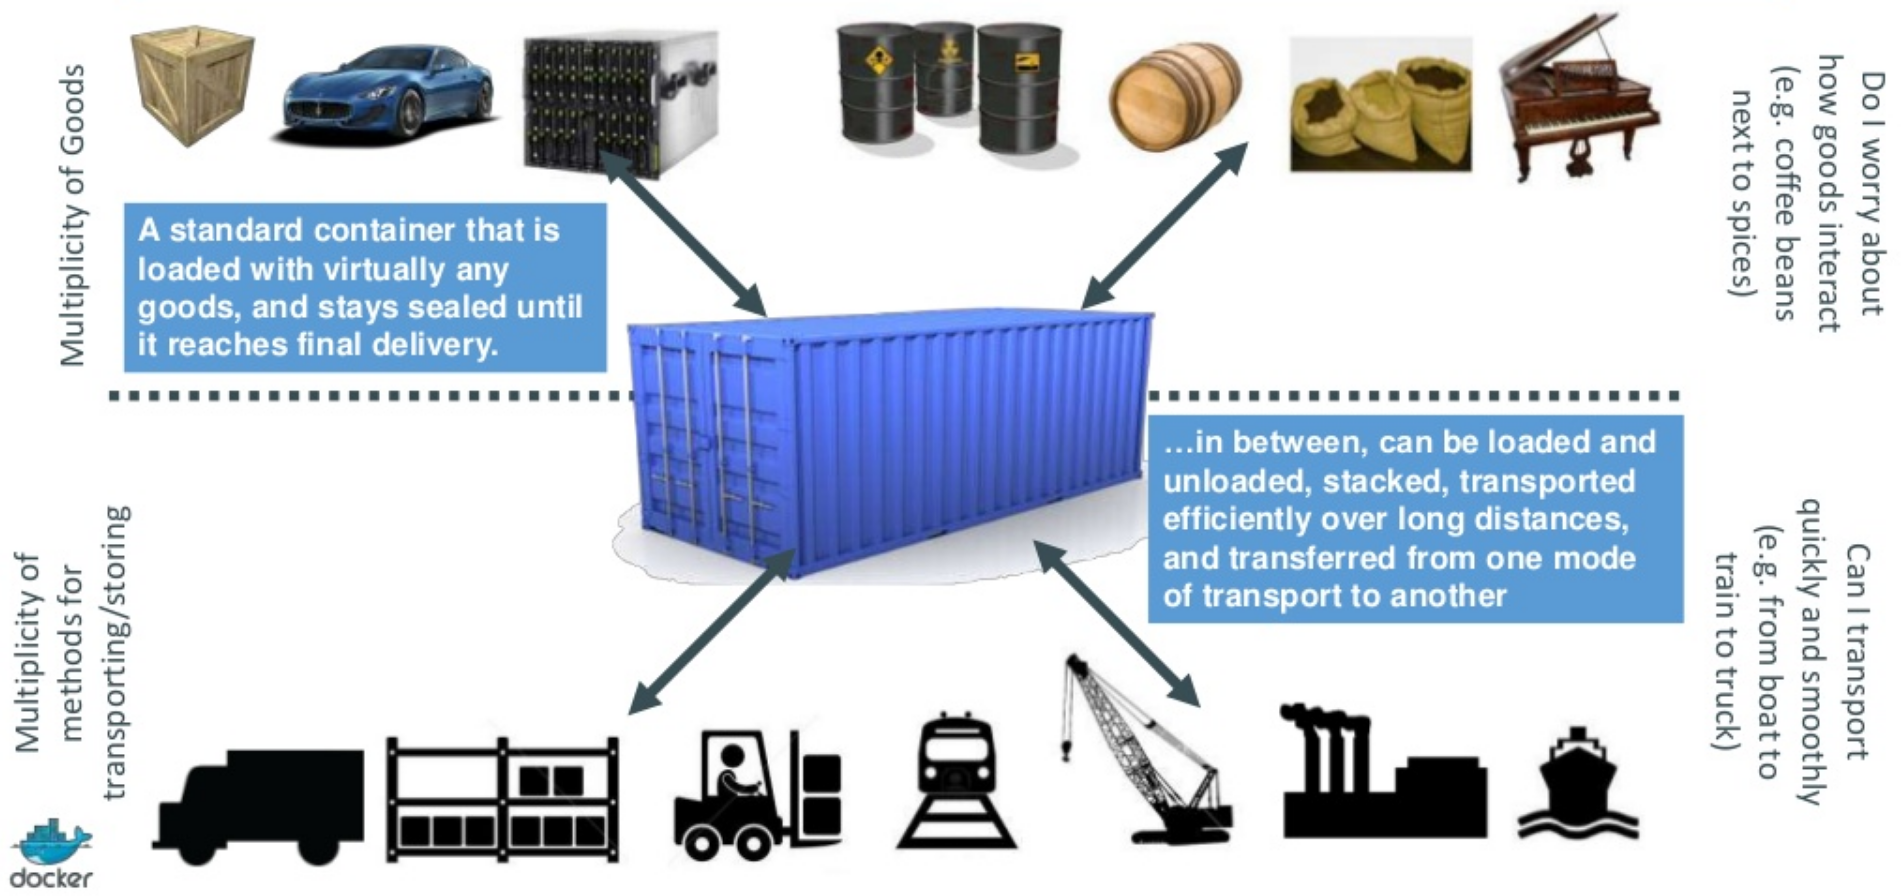
\includegraphics[width=0.80\paperwidth]{docker-zomato/images/cargo_container.png}}
%            }
%            \only<5-1> {
%             \begin{block}{Docker is just that}\end{block}
%                \makebox[\textwidth]{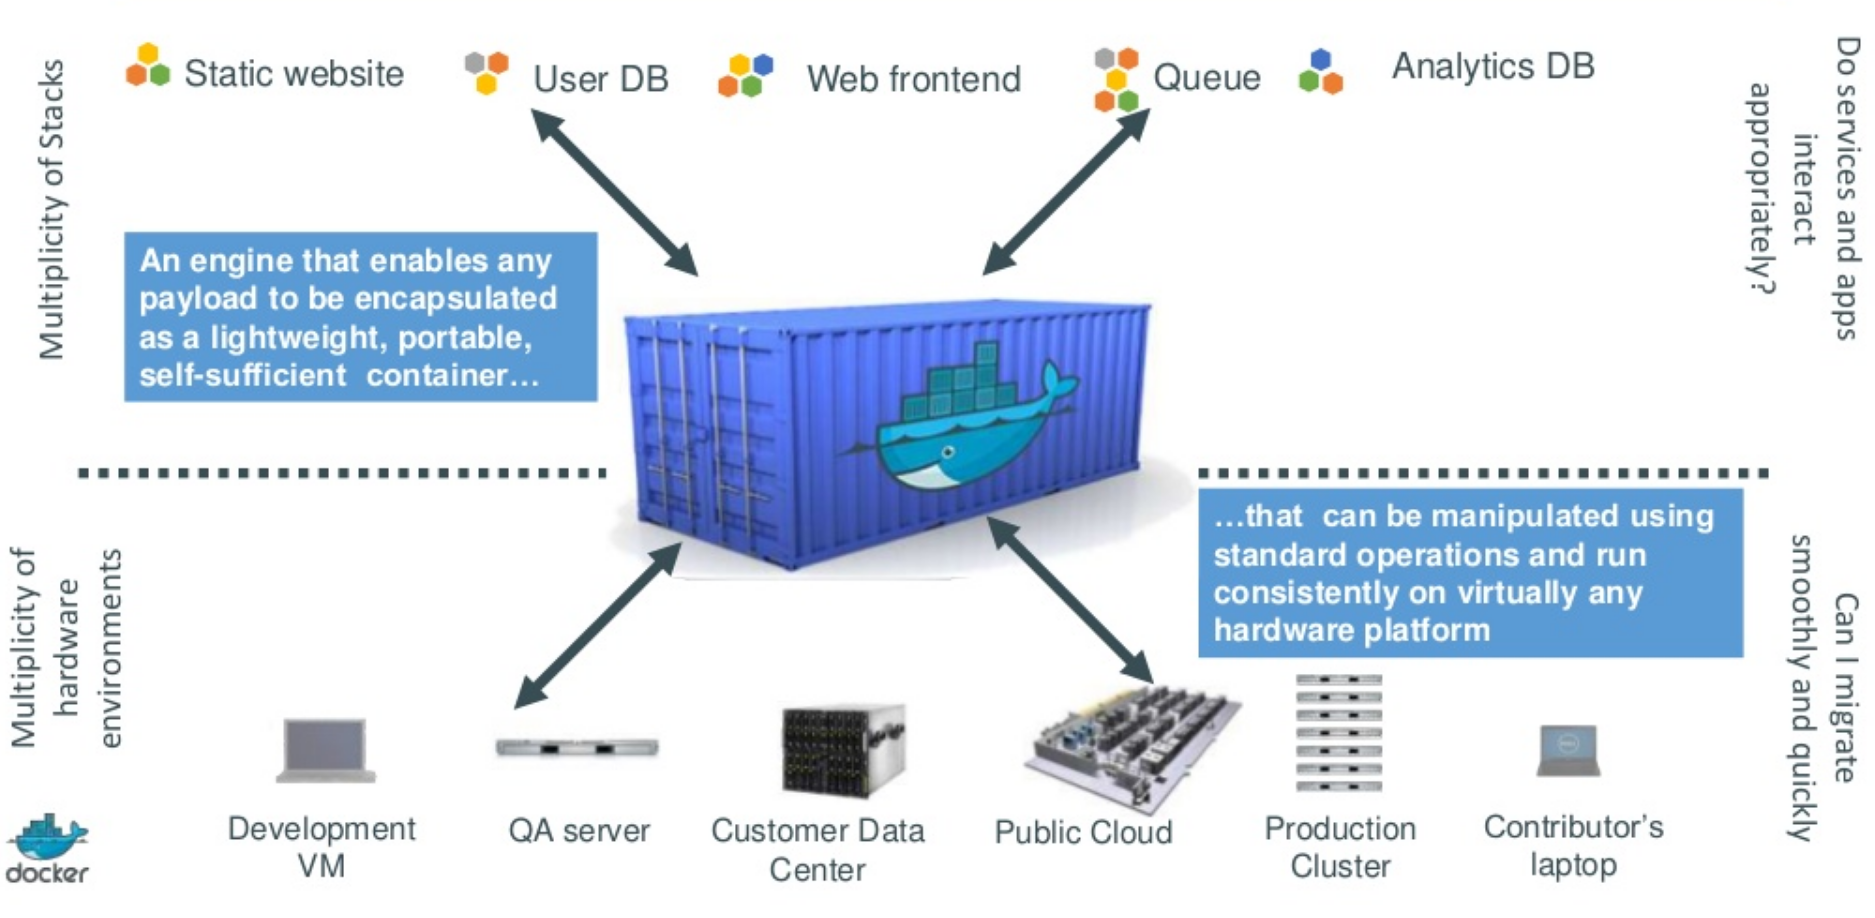
\includegraphics[width=0.80\paperwidth]{docker-zomato/images/matrix_doc.png}}
%            }
%            \only<6-1> {
%             \begin{block}{The solution to matrix of hell}\end{block}
%            \makebox[\textwidth]{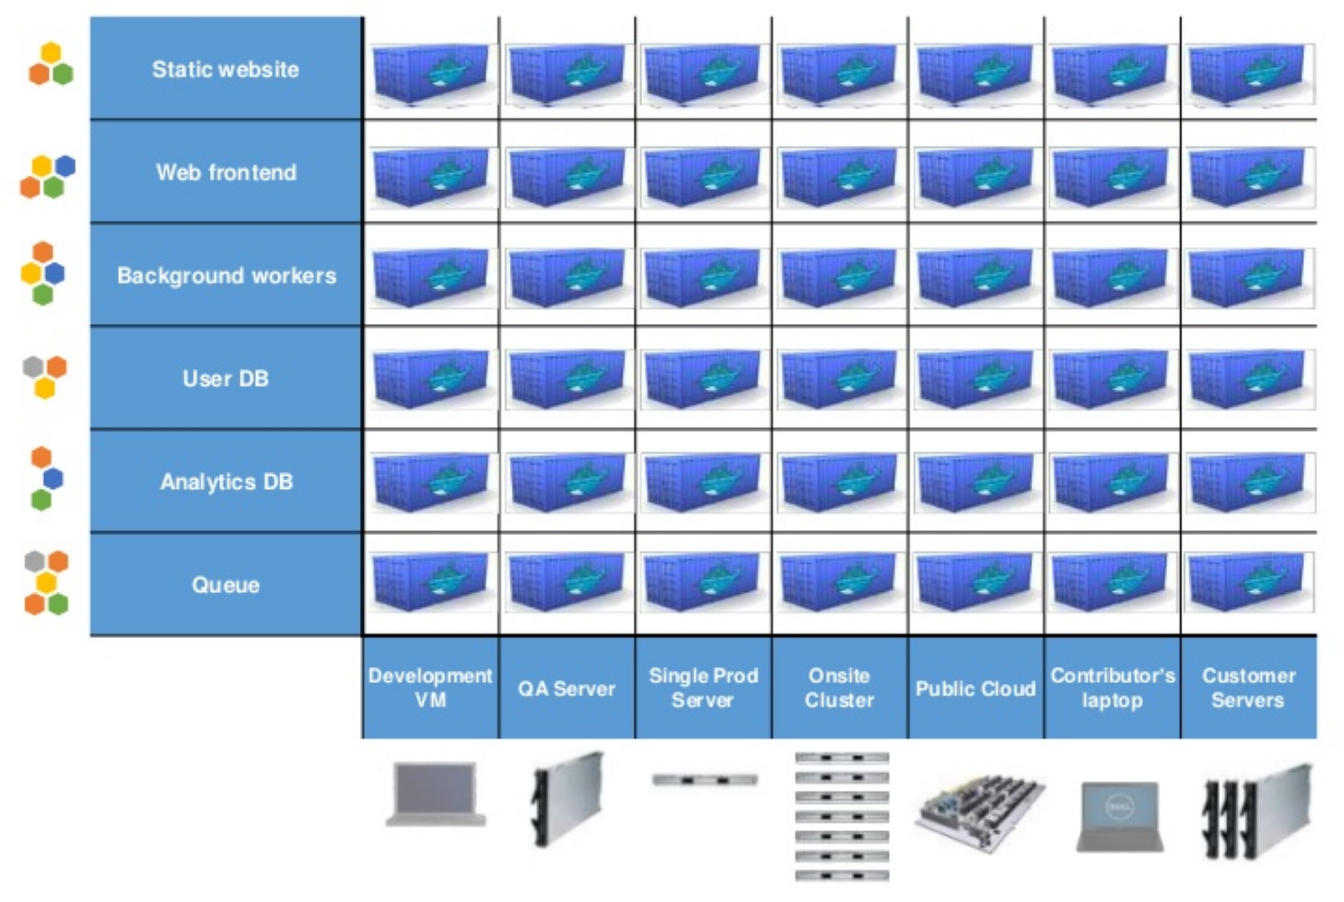
\includegraphics[width=0.80\paperwidth]{docker-zomato/images/matrix_sol.png}}
%            }
%        \end{itemize}
%    \end{frame}
    \begin{frame}
        \frametitle{The Problem that dotCloud wanted to solve}
        \framesubtitle{Matrix of Hell}
        \begin{center}
            \makebox[\textwidth]{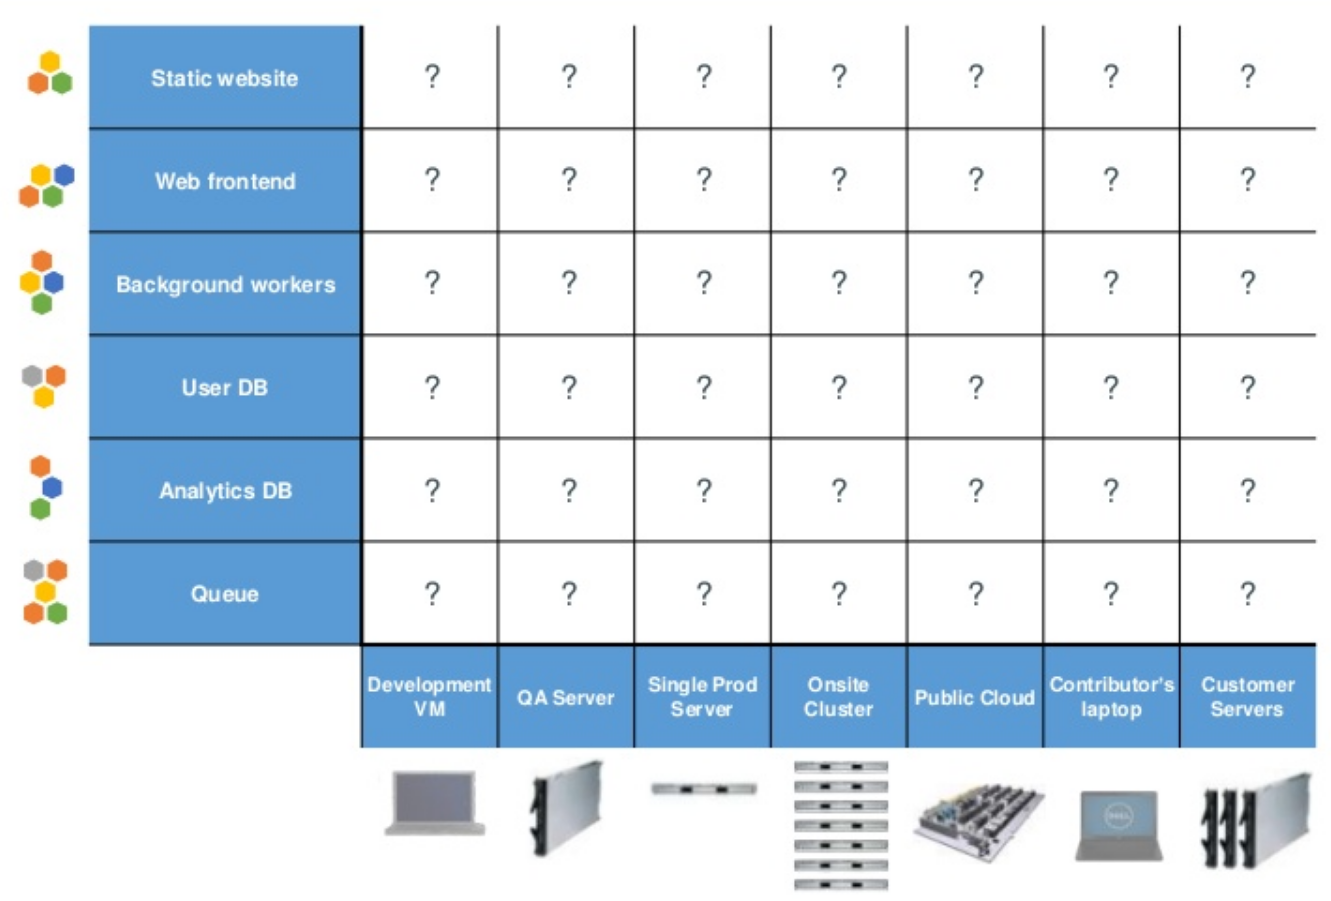
\includegraphics[width=0.80\paperwidth]{docker-zomato/images/matrix_prob.png}}
        \end{center}
    \end{frame}

    \begin{frame}
        \frametitle{Docker wasn't the first}
        \begin{center}
            \makebox[\textwidth]{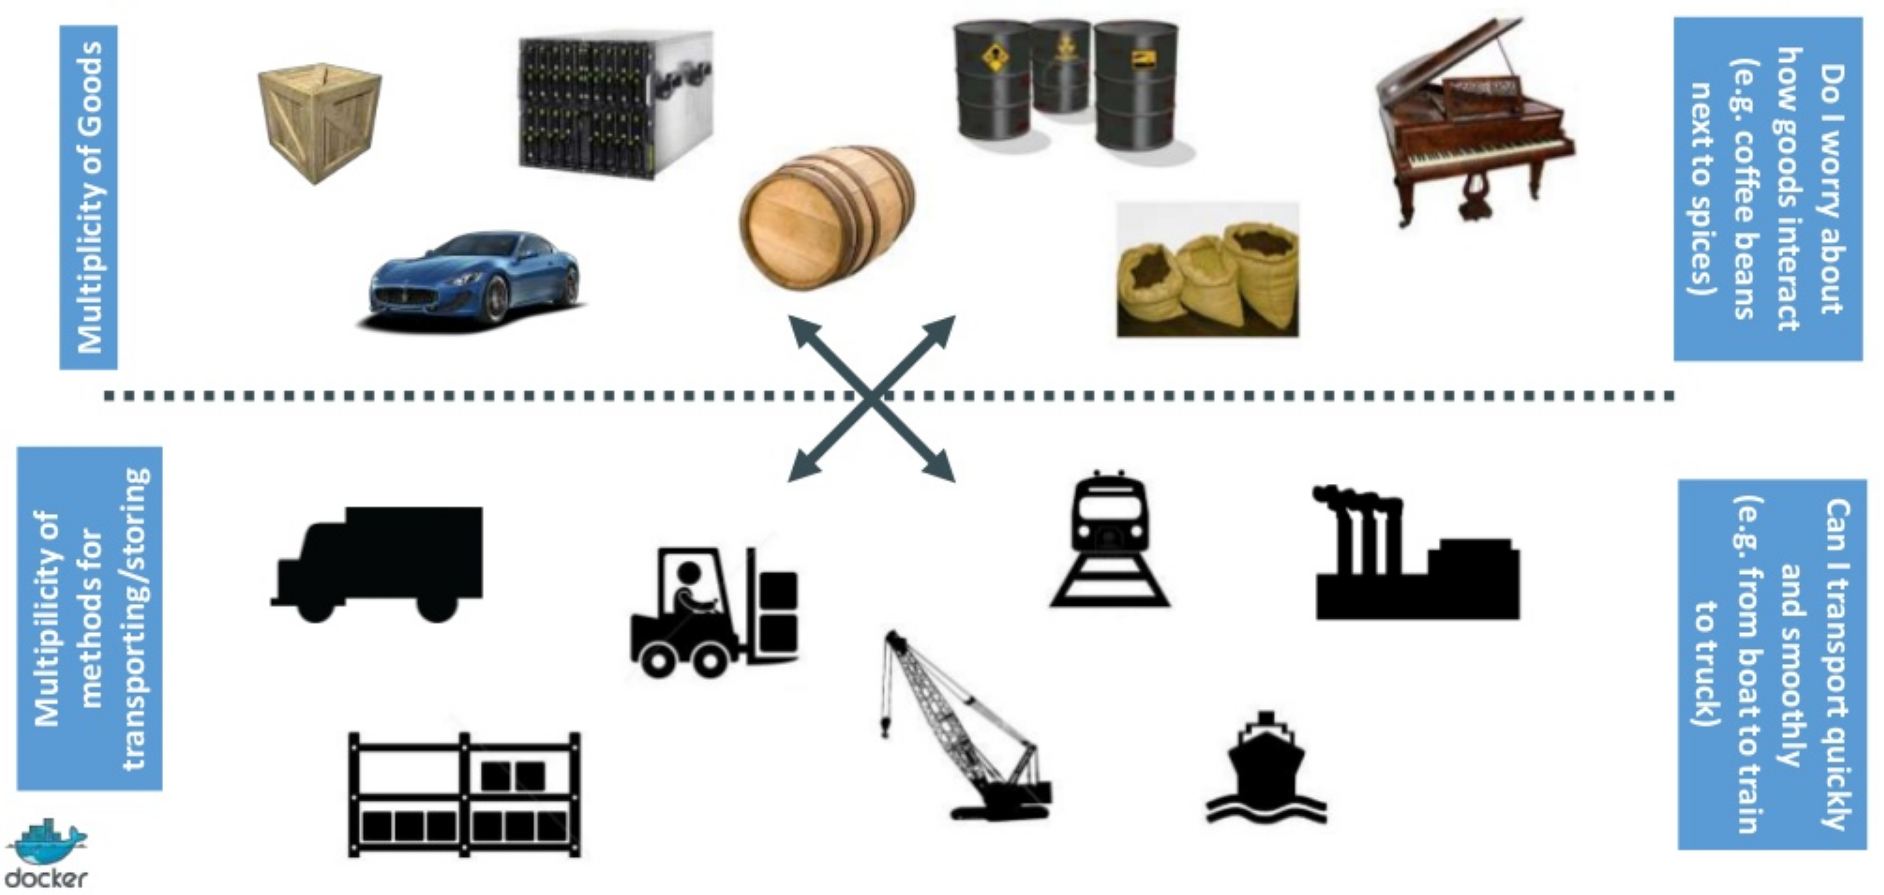
\includegraphics[width=0.80\paperwidth]{docker-zomato/images/cargo_prob.png}}
        \end{center}
    \end{frame}

    \begin{frame}
        \frametitle{Similar matrix of hell}
        \begin{center}
            \makebox[\textwidth]{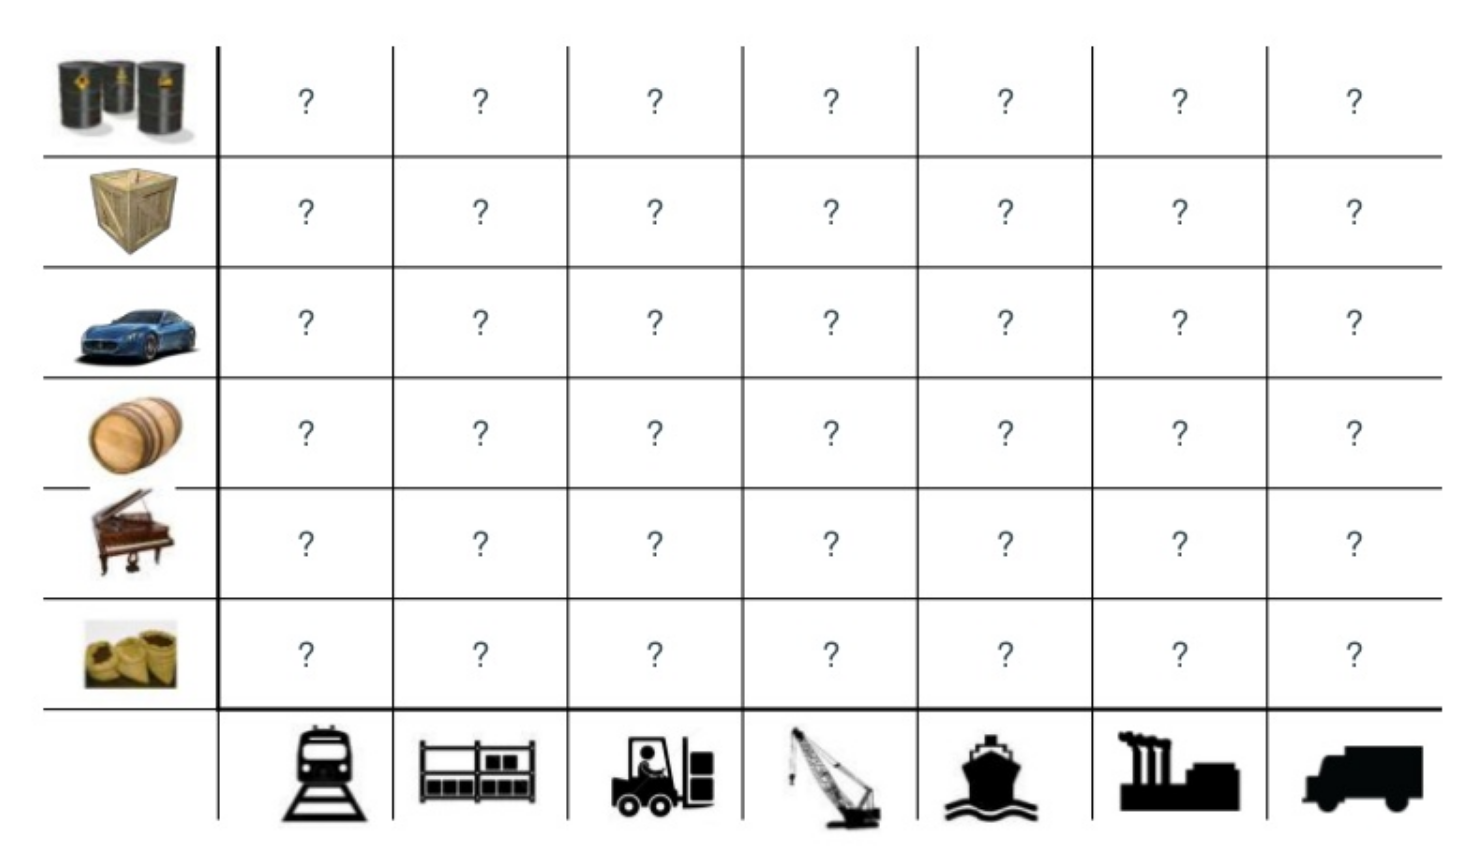
\includegraphics[width=0.80\paperwidth]{docker-zomato/images/cargo_matrix.png}}
        \end{center}
    \end{frame}

    \begin{frame}
        \frametitle{Cargo Industry's Solution - Containers}
        \begin{center}
            \makebox[\textwidth]{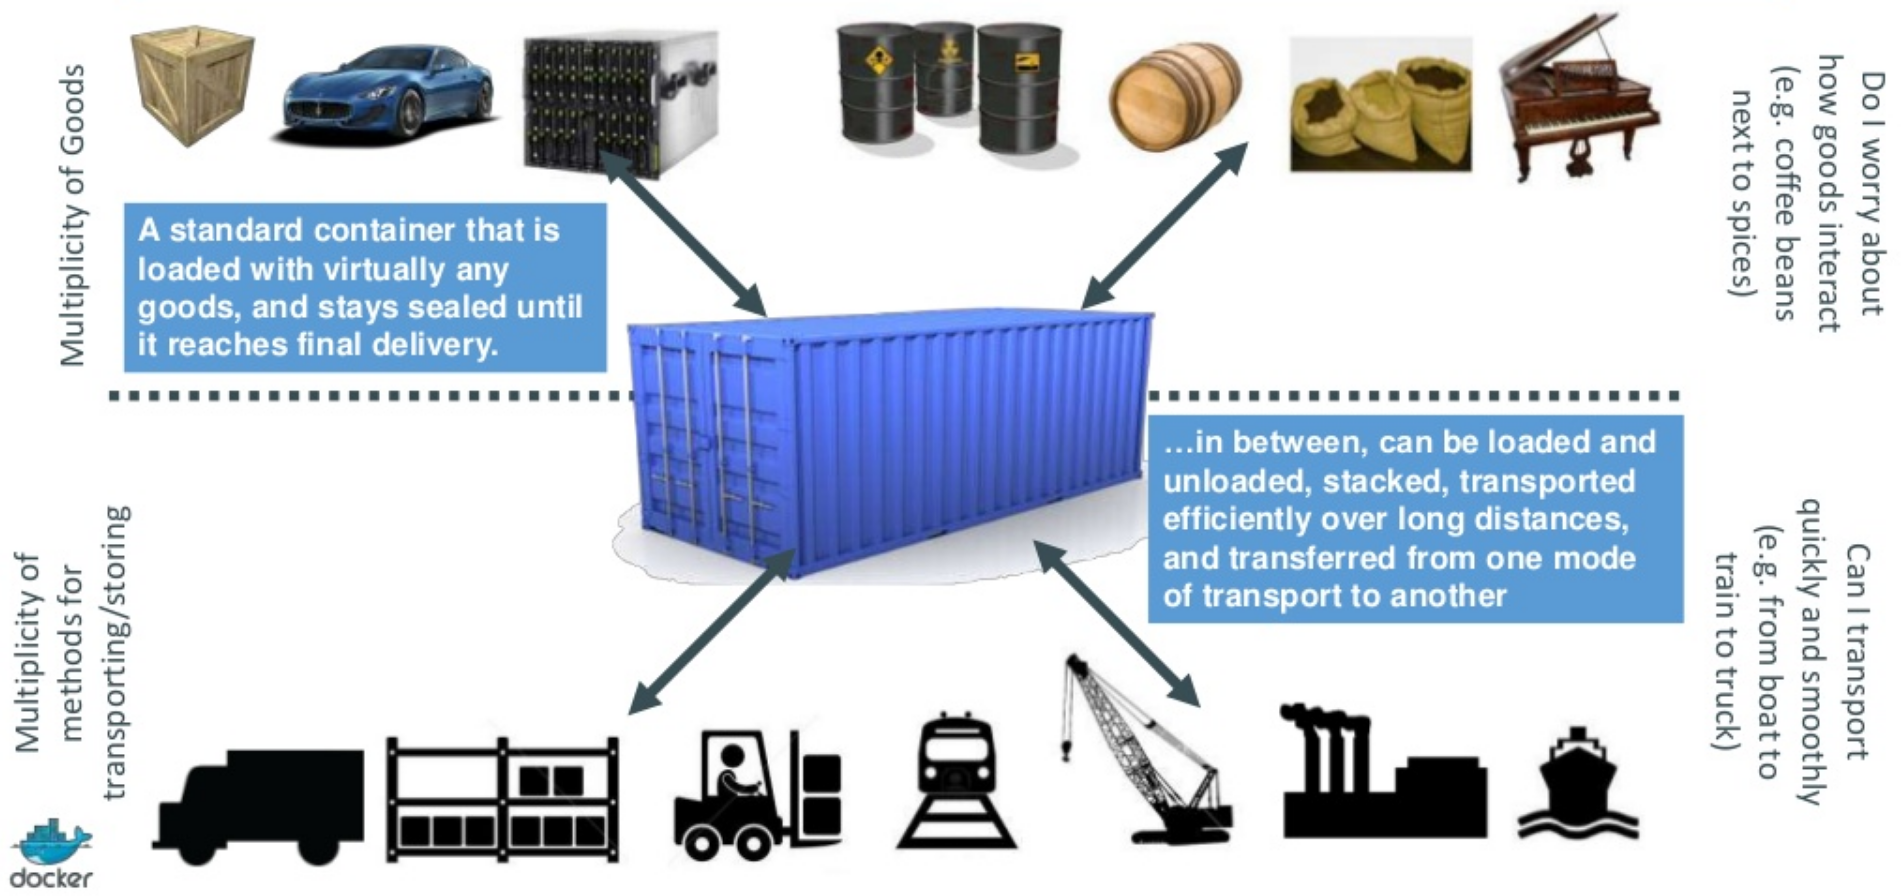
\includegraphics[width=0.80\paperwidth]{docker-zomato/images/cargo_container.png}}
        \end{center}
    \end{frame}

    \begin{frame}
        \frametitle{Docker is just that}
        \begin{center}
            \makebox[\textwidth]{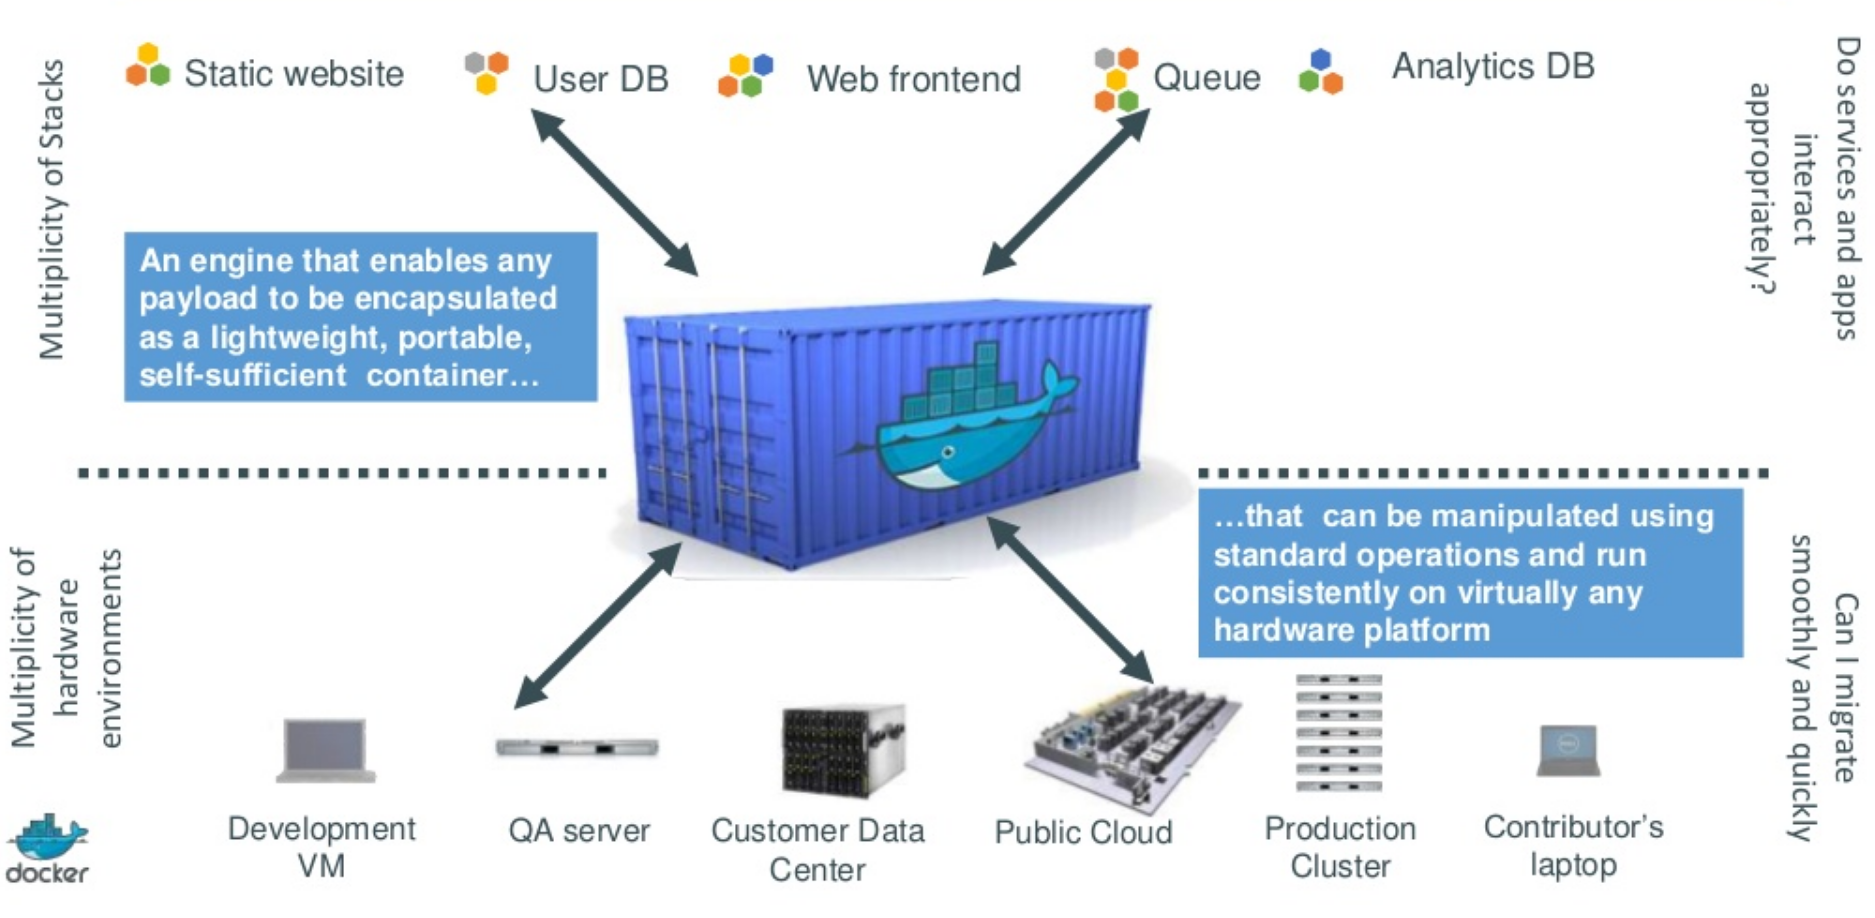
\includegraphics[width=0.80\paperwidth]{docker-zomato/images/matrix_doc.png}}
        \end{center}
    \end{frame}

    \begin{frame}
        \frametitle{The solution to matrix of hell}
        \begin{center}
            \makebox[\textwidth]{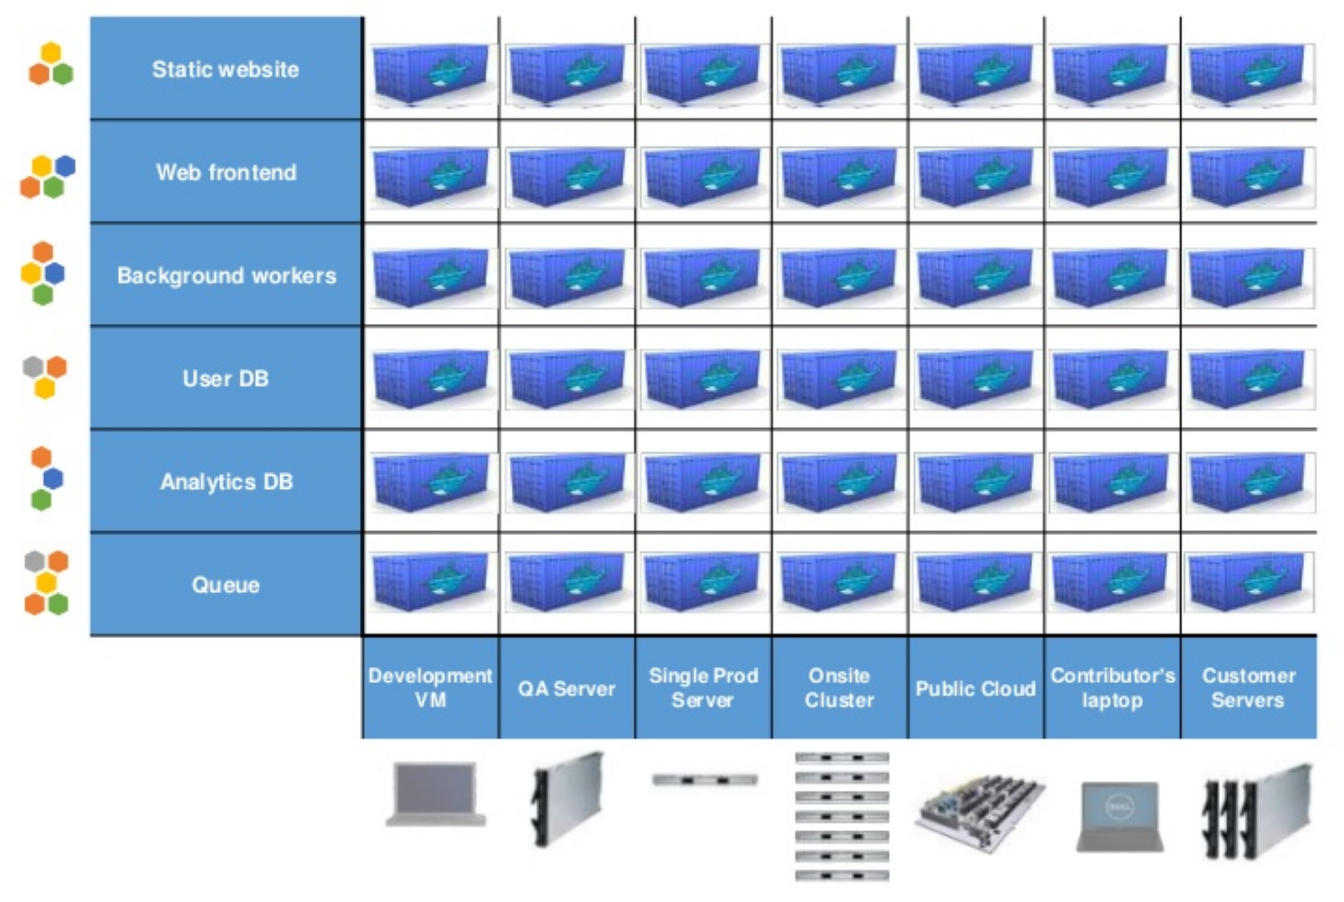
\includegraphics[width=0.80\paperwidth]{docker-zomato/images/matrix_sol.png}}
        \end{center}
    \end{frame}


    \section{What is Docker}\label{sec:whatIsDocker}
    \begin{frame}
        \frametitle{What is docker?}
        \begin{columns}[t]
            \begin{column}{0.40\textwidth}
                \begin{itemize}[<+->]
                    \item \href{https://www.docker.com/what-docker}{Docker.io} says: \\
                          An engine that automates the deployment of any application as a lightweight,
                          portable, self-sufficient container that will run virtually anywhere.

                    \item Technically, Docker is AMIs on diet, \\
                          or cgroups on steroids.
                \end{itemize}
            \end{column}
            \begin{column}{0.40\textwidth}
                \begin{center}
                    \makebox[0.40\textwidth]{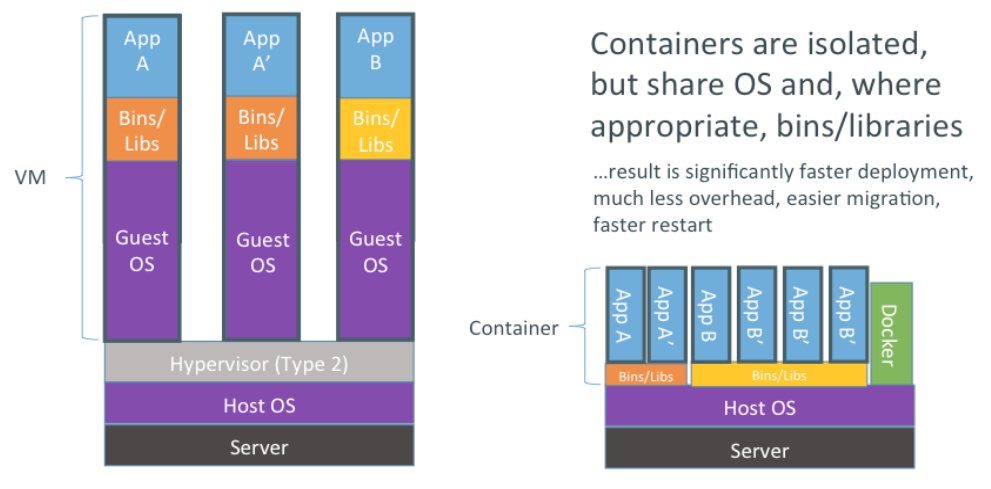
\includegraphics[width=0.40\paperwidth]{docker-zomato/images/vm_vs_container.png}}
                \end{center}
            \end{column}
        \end{columns}
    \end{frame}

    \begin{frame}
        \frametitle{Why are docker containers lightweight?}
        \begin{center}
            \makebox[0.80\textwidth]{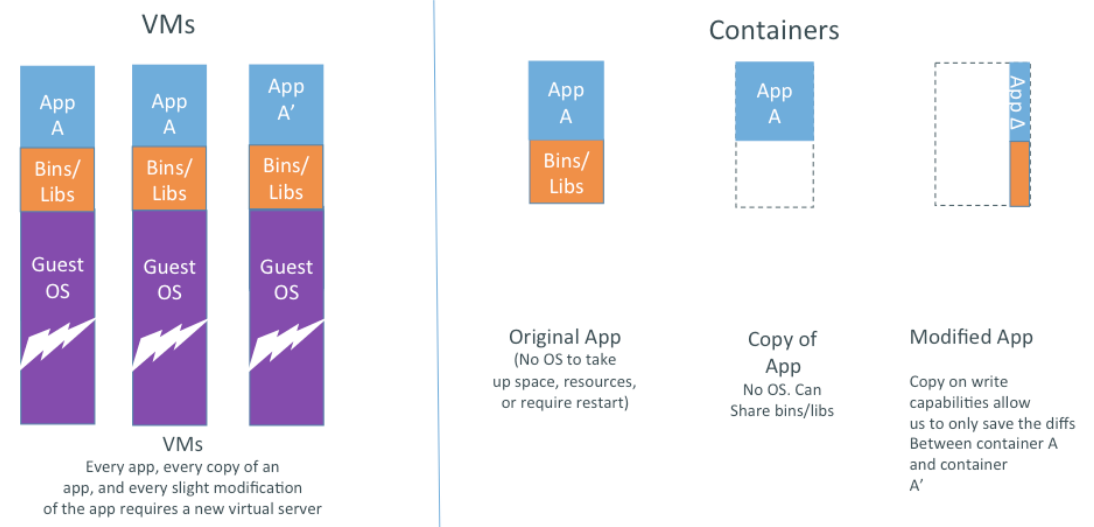
\includegraphics[width=0.80\paperwidth]{docker-zomato/images/lightweight.png}}
        \end{center}
    \end{frame}


    \subsection{Benefits}\label{subsec:separationOfConcerns}
    \begin{frame}
        \frametitle{Version Control for deployment}
        \framesubtitle{Think of docker as git for deployment}
        \begin{center}
            \begin{tabular}{ | l | l | l | }
                \hline
                \textbf{Docker} & \textbf{Git} & \textbf{Description} \\
                \hline
                Image & Repository & Collection of commits \\
                DockerHub & GitHub & Popular hosting service \\
                Container & Clone & Used for local execution \\
                \hline
            \end{tabular}
        \end{center}
        Dockerizing your app, enables anyone to reproduce it with no effort. \\
        This is exactly what git (and github) did.
    \end{frame}

    \begin{frame}
        \frametitle{Separation of concerns}
        \begin{center}
            \makebox[\textwidth]{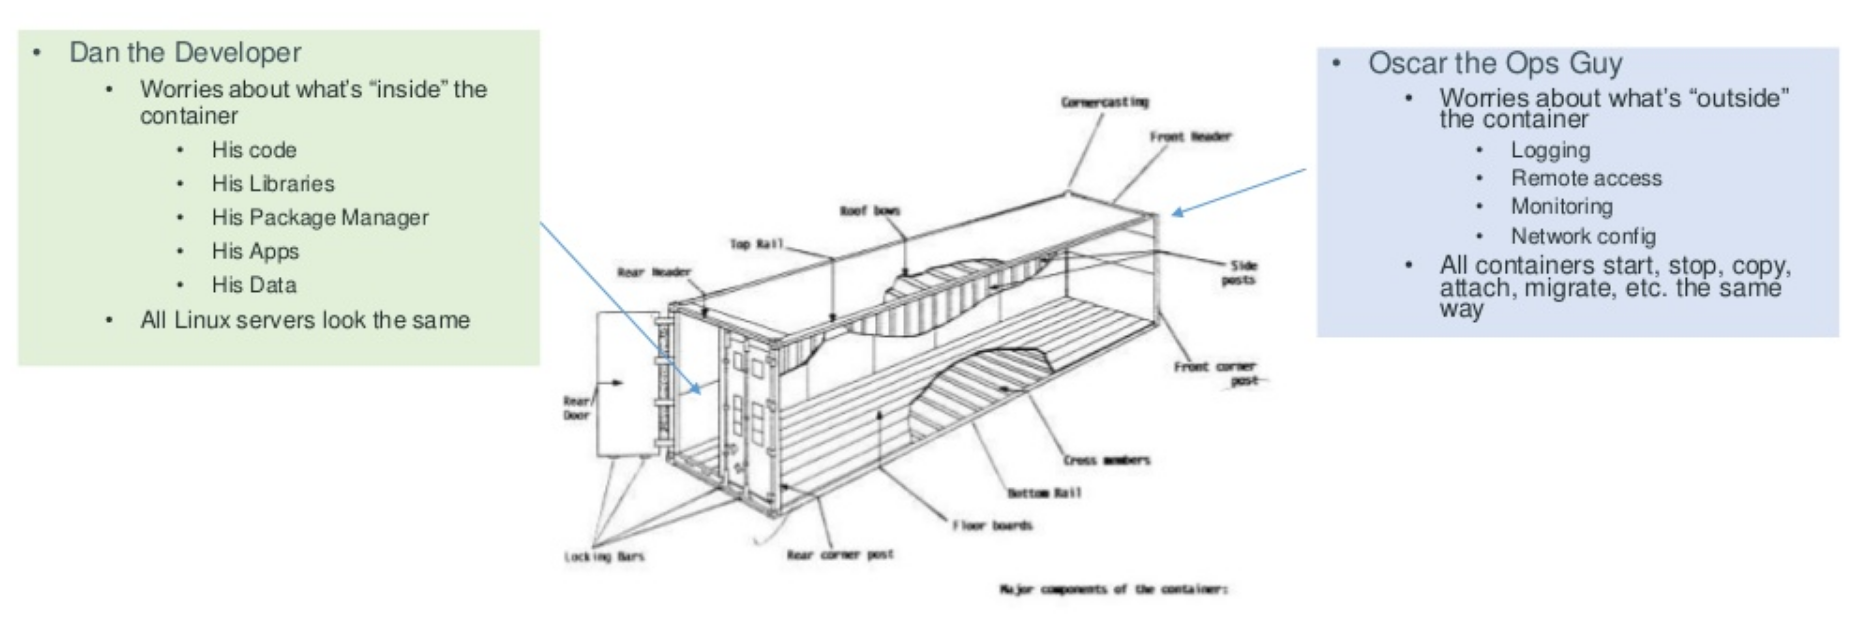
\includegraphics[width=\paperwidth]{docker-zomato/images/soc.png}}
        \end{center}
        %        \only<1>{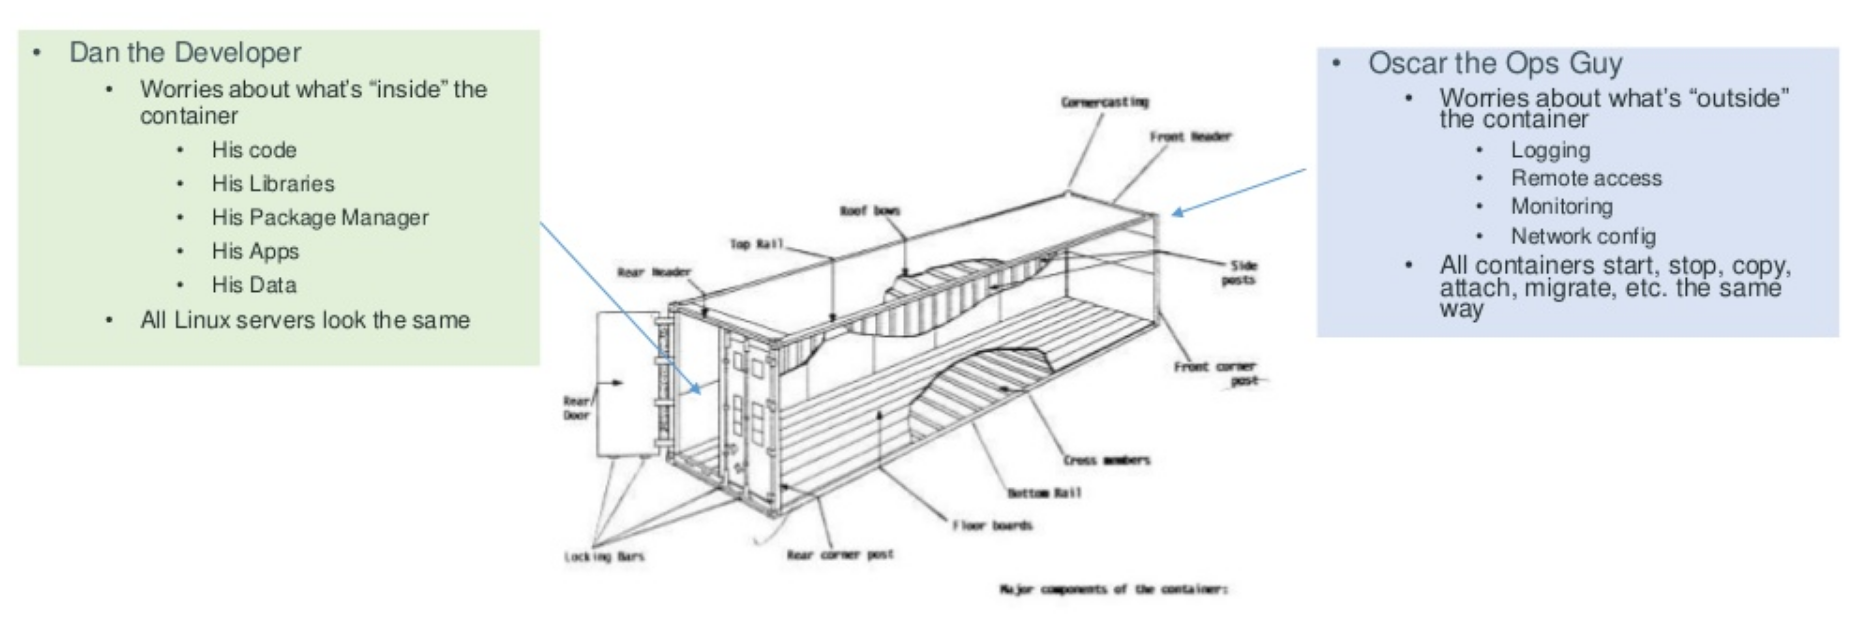
\includegraphics[width=\paperwidth]{docker-zomato/images/soc.png}}
    \end{frame}


    \section{Development with Docker}\label{sec:developmentWithDocker}
    \begin{frame}
        \frametitle{Basic Workflow}
        \framesubtitle{Brief intro to the commands}
        \begin{itemize}[<+->]
            \item Find an image - docker search nginx
            \only<1-1> {\makebox[0.7\textwidth]{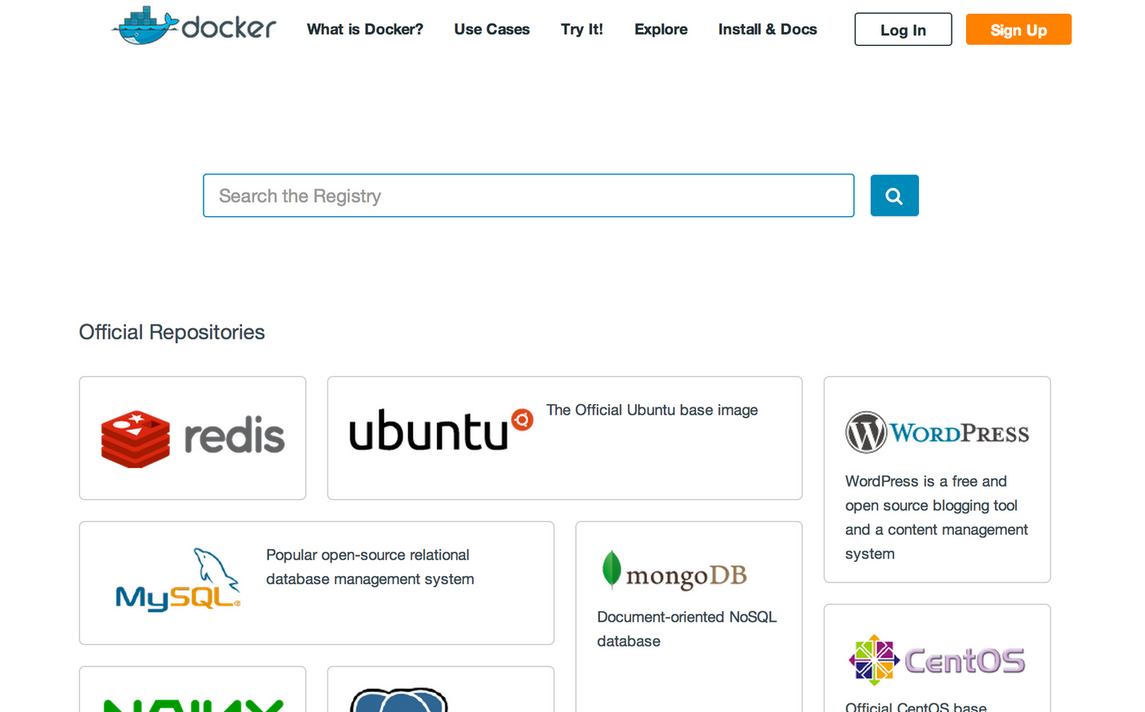
\includegraphics[width=0.6\paperwidth]{docker-zomato/images/hub.png}}}
            \item Pull the image - docker pull nginx
            \item Run the image in a container on the host - docker run -it nginx --name demo-nginx
            \item Stop the container - docker stop/rm demo-nginx
            \item Remove the image - docker rmi nginx
        \end{itemize}
    \end{frame}

    \subsection{CLI Usage}\label{subsec:cliUsage}
    \begin{frame}
        \begin{center}
            docker run -it -p 8080:80 \\
            -v `pwd`/nonsvn/nginx/conf.d:/etc/nginx/conf.d \\
            -v `pwd`/nonsvn/nginx .conf:/etc/nginx.conf \\
            nginx
        \end{center}
        \begin{itemize}[<+->]
            \item \textbf{-it}: Interactive (Keep STDIN open even if not attached), TTY (Allocate a pseudo-TTY)
            \item \textbf{-p 8080:80}: Port Mapping
            \item \textbf{-v `pwd`/nonsvn/nginx/conf.d:/etc/nginx/conf.d}: Volume Mapping
            \item \textbf{-v `pwd`/nonsvn/nginx.conf:/etc/nginx.conf}: Volume Mapping (files)
        \end{itemize}
    \end{frame}

%    \begin{frame}
%        Rule of thumb: One container for each process
%    \end{frame}

    \subsection{Demo - SQL}\label{subsec:demo-Sql}
    \begin{frame}
        \frametitle{Demo - SQL}
        \framesubtitle{Running a nginx server in 10 secs}
        \begin{figure}[h!]
            \centering
%            \movie[label=show3,height=0.75\textheight,width=0.85\textwidth,poster,autostart,showcontrols,loop]
            {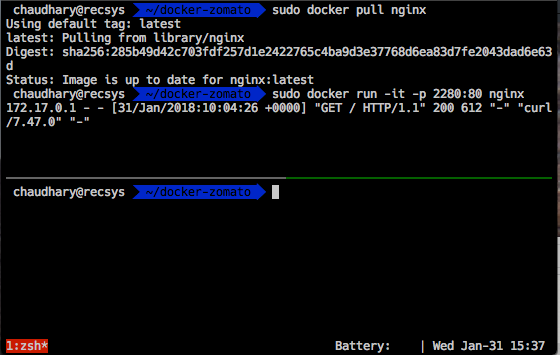
\includegraphics[height=0.75\textheight,width=0.85\textwidth]{docker-zomato/images/nginx.png}}
%            {videos/nginx.mp4}
            \caption{caption}
        \end{figure}
    \end{frame}
    \subsection{Demo - Spark Cluster}\label{subsec:demo-SparkCluster}
    \begin{frame}
        \frametitle{Demo - Spark Cluster}
        \framesubtitle{Running a spark cluster in 10 secs}
        \begin{figure}[h!]
            \centering
            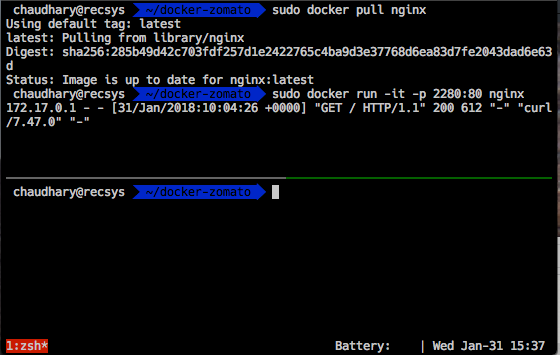
\includegraphics[height=0.75\textheight,width=0.85\textwidth]{docker-zomato/images/nginx.png}
            \caption{caption}
        \end{figure}
    \end{frame}

    \subsection{Project Workflow}\label{subsec:basicWorkflow}
    \begin{frame}
        \frametitle{Development Workflow when using docker}
        \begin{center}
            \makebox[\textwidth]{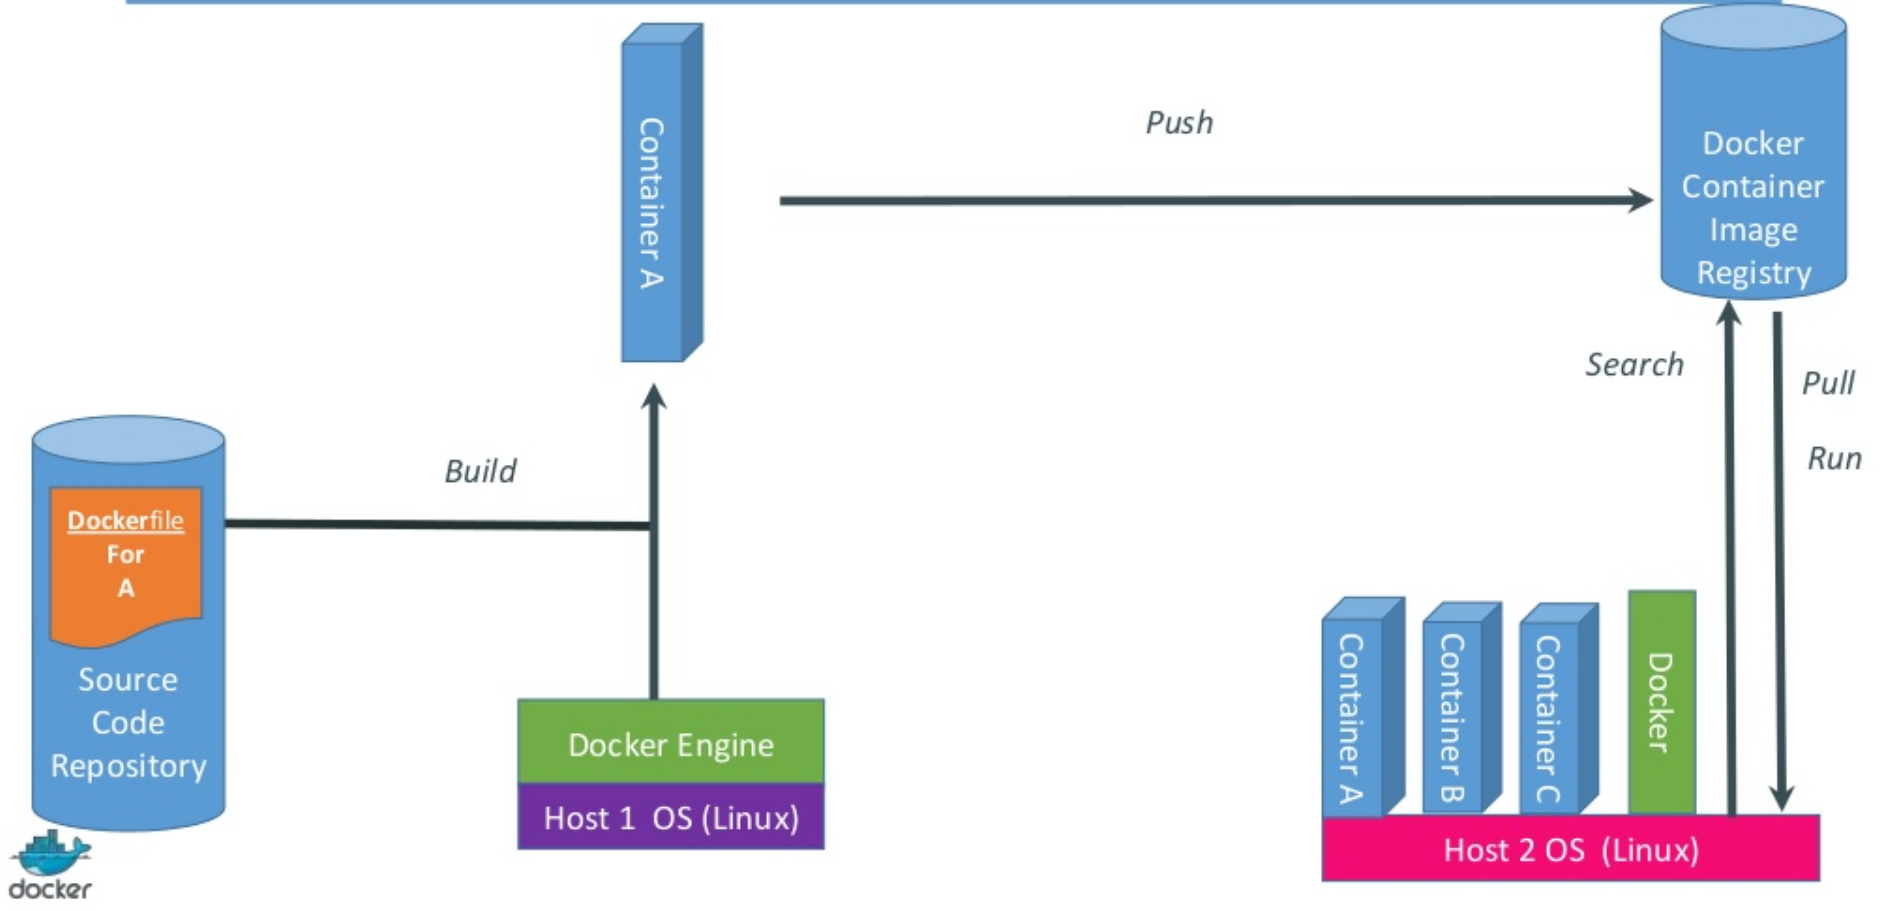
\includegraphics[width=0.80\paperwidth]{docker-zomato/images/workflow_fc.png}}
        \end{center}
    \end{frame}

    \subsection{Dockerfile}\label{subsec:dockerfile}
    \begin{frame}
        \frametitle{Dockerfile}
        Here is a dummy Dockerfile:

        \begin{center}
            \makebox[\textwidth]{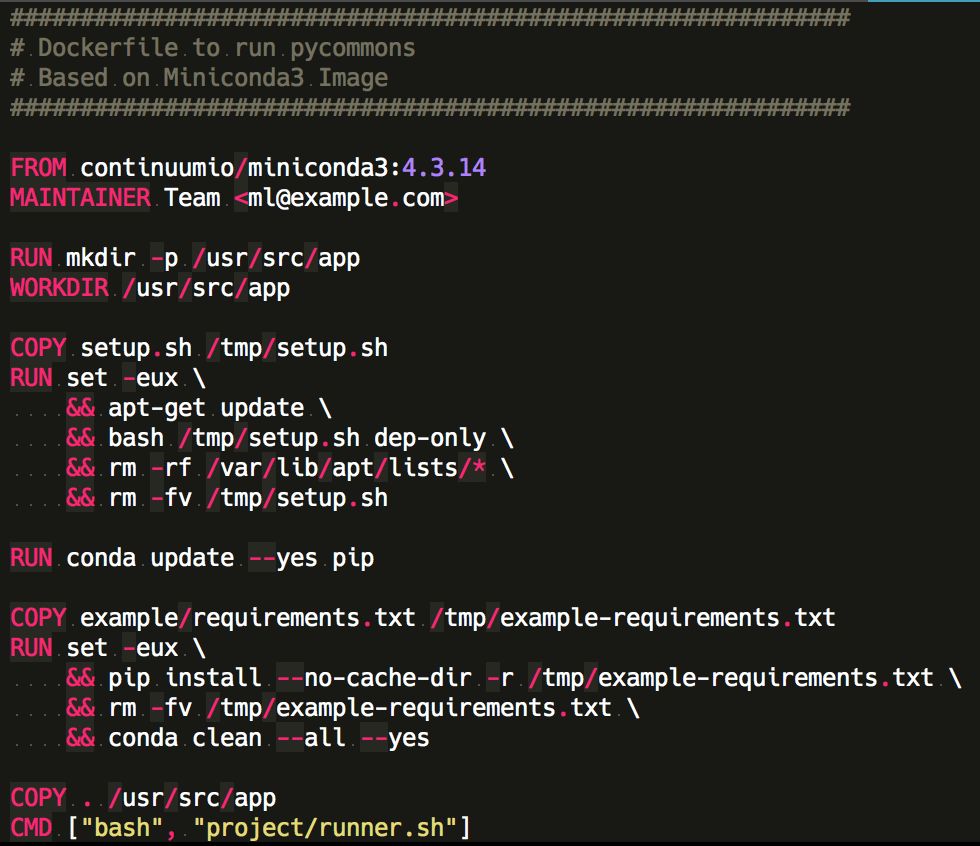
\includegraphics[height=0.60\paperheight]{docker-zomato/images/dockerfile.png}}
        \end{center}
    \end{frame}

    \subsection{Image Inheritance}\label{subsec:inheritance}
    \begin{frame}
        \frametitle{Extending other images}
        \framesubtitle{Inheritance}
        \begin{center}
            \makebox[\textwidth]{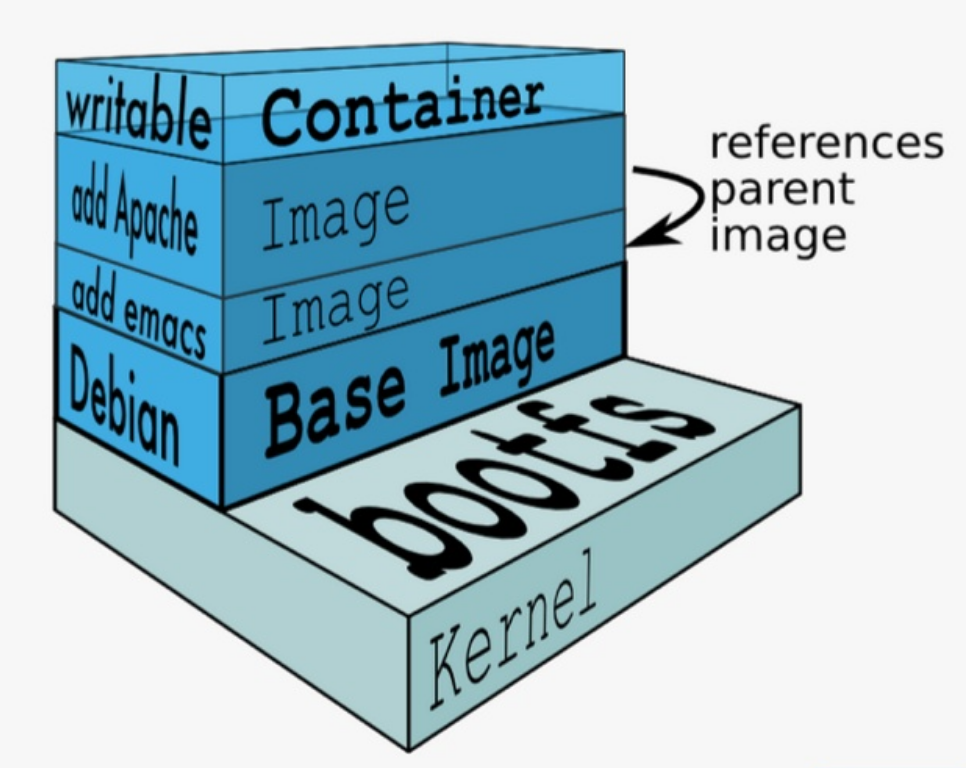
\includegraphics[width=0.80\paperwidth]{docker-zomato/images/image_inheritence.png}}
        \end{center}
    \end{frame}

    \section{Multi-Container Projects}\label{sec:multi-containerProjects}
    \begin{frame}
        Real life applications are complicated.
        They need more that just one webapp.

        \begin{itemize}
            \item Docker Compose
%                \subitem Service Discovery
%                \subitem NAT
            \item Kubernetes
            \item Elastic Beanstalk
        \end{itemize}
    \end{frame}


    \section{Credits}\label{sec:credits}
    \begin{frame}
        \begin{center}
            Thanks
        \end{center}

        \begin{itemize}
            \item http://slides.com/atbaker/docker-101
            \item https://www.slideshare.net/Docker/docker-101-introduction-to-docker
            \item https://www.slideshare.net/dotCloud/docker-intro-november
        \end{itemize}
    \end{frame}

\end{document}
